% Chapter 4, Topic _Linear Algebra_ Jim Hefferon
%  http://joshua.smcvt.edu/linearalgebra
%  2001-Jun-12
\topic{Projective Geometry}
\index{projective geometry|(}
There are geometries other than the familiar Euclidean one.
One such geometry arose when artists observed
that what a viewer sees is not necessarily what is there.
As an example, here is Leonardo da Vinci's 
\textit{The Last Supper}.\index{da Vinci, Leonardo}\index{Last Supper@\textit{Last Supper}}
% From http://upload.wikimedia.org/wikipedia/commons/7/77/DaVinci_LastSupper_high_res_2_nowatmrk.jpg
\begin{center} 
  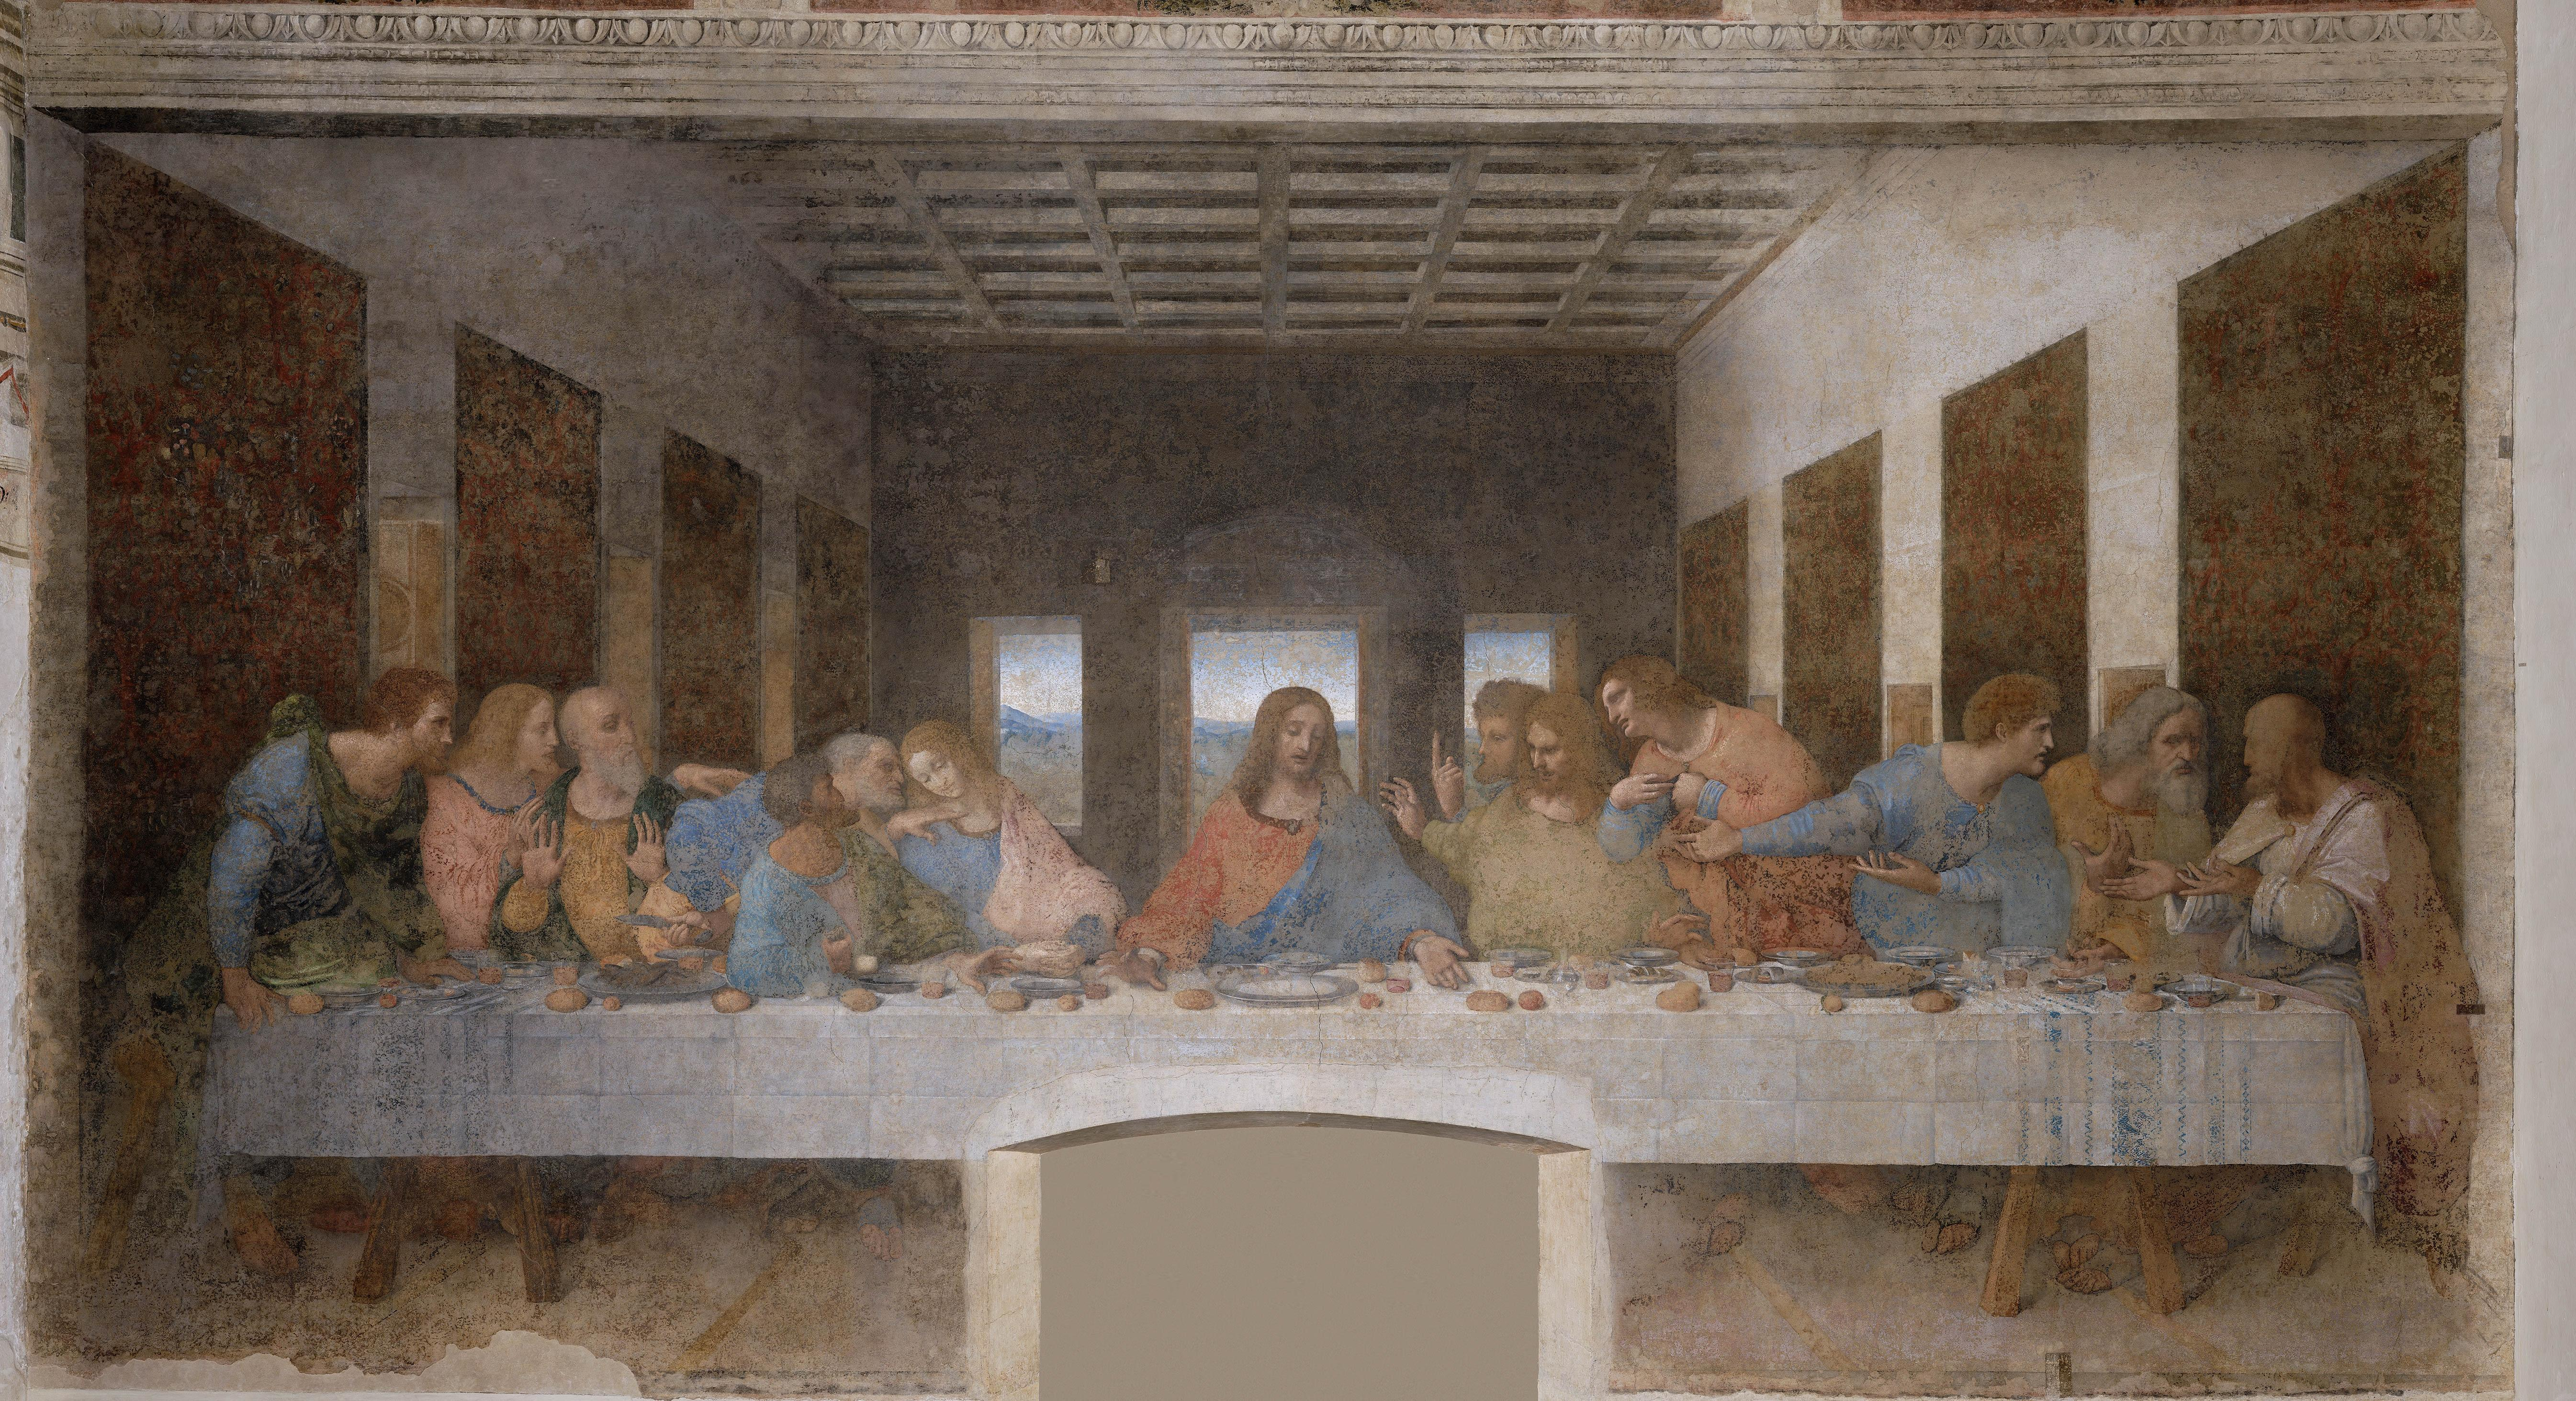
\includegraphics[width=.6\textwidth]{LastSupper.jpg}
\end{center}
Look at where the ceiling meets the left and right walls.
In the room those lines are parallel but 
da~Vinci has painted lines that, if extended, would intersect.
The intersection is the 
\definend{vanishing point}.\index{vanishing point}\index{projection!central!vanishing point}
This aspect of perspective is familiar as an image of 
railroad tracks that appear to converge at the horizon.

Da~Vinci has adopted a model of how we see.
% of how
% we project the three dimensional scene to a two dimensional image.
Imagine a person viewing a room.
From the person's eye, in every direction,
carry a ray outward until it intersects something, such
as a point on the line where the wall meets the ceiling.
This first intersection point is what the person sees in that direction.
Overall what the person sees is the collection of three-dimensional
intersection points
projected to a common two dimensional image. 
\begin{center}
  \includegraphics[scale=.8]{ch4.5}
\end{center}
This is a 
\emph{central projection}\index{projection!central}\index{central projection} 
from a single point.
As the sketch shows, this projection is not orthogonal
like the ones we have seen earlier 
because the line
from the viewer to~$C$ is not orthogonal to the image plane.
(This model is only an approximation\Dash it does not take into
account such factors as
that we have binocular vision or that our brain's processing 
greatly affects what we perceive. 
Nonetheless the model is interesting,
both artistically and mathematically.)

The operation of  
central projection preserves some geometric 
properties, for instance lines project to lines.
However, it fails to preserve some others.
One example is that equal 
length segments can project to segments of unequal length 
(above, $AB$ is longer than $BC$ because the
segment projected to $AB$ is closer to the viewer and 
closer things look bigger).
The study of the effects of central projections is projective geometry.

There are three cases of central projection.
The first is the projection done by a movie projector.
\begin{center}
  \includegraphics{ch4.6}
\end{center}
We can think that each source point is pushed from the domain plane~$S$
outward to the image plane~$I$.
The second case of projection is that of the artist
pulling the source back to a canvas.
\begin{center}
  \includegraphics{ch4.7}
\end{center}
The two are different because first $S$ is in the middle
and then $I$.
One more configuration can happen, with $P$ in the middle. 
An example of this is when we use a pinhole to shine the 
image of a solar eclipse onto a paper.
\begin{center}
  \includegraphics{ch4.8}
\end{center}

Although the three are not exactly the same,  
they are similar.
We shall say that 
each is a central projection by $P$ of
$S$ to $I$.
We next look at three models of central projection, 
of increasing abstractness but
also of increasing uniformity.
The last model will bring out the linear algebra.

%To illustrate some of the geometric effects of these projections,  
Consider again the effect of railroad tracks  
that appear to converge to a point.
Model this with parallel lines in a domain plane~$S$
and a projection via a $P$ to a codomain plane~$I$. 
(The gray lines shown are parallel to the $S$ plane and to the~$I$ plane.)
\begin{center}
  \includegraphics{ch4.9}
\end{center}
This single setting shows all three projection cases.
The first picture below shows $P$ acting as a movie projector by pushing
points from part of $S$ out to image points on the lower half of $I$.
The middle picture shows $P$ acting as the artist by 
pulling points from another part of $S$ back to  
image points in the middle of $I$.
In the third picture $P$ acts as the pinhole, projecting points from $S$
to the upper part of $I$.
This third picture is the trickiest\Dash the points that are
projected near to the vanishing point are the ones that are 
far out on the lower left of $S$. 
Points in $S$ that are near to the vertical gray line
are sent high up on $I$.
\begin{center}
  \includegraphics{ch4.10}
\hfil
  \includegraphics{ch4.11}
\hfil
  \includegraphics{ch4.12}
\end{center}

There are two awkward things here.
First, neither of the two points in the domain
nearest to the vertical gray line (see below) has an image 
because a projection from those two is along the
gray line that is parallel to the codomain plane
(we say that these two are projected to infinity).
The second is that 
the vanishing point in $I$
isn't the image of any point from $S$ 
because a projection to this point would be along the gray line
that is parallel to the domain plane
(we say that the vanishing point is the image of a projection 
from infinity).
\begin{center}
  \includegraphics{ch4.13}
\end{center}

For a model that eliminates this awkwardness, 
cover the projector $P$ with a hemispheric dome.
In any direction, defined by a line through the origin, project anything 
in that direction to the single spot on the dome where the line intersects.
This includes projecting things on the line between $P$ and the dome, 
as with the movie projector.
It includes projecting things on the line further from $P$ than the dome,
as with the painter.
More subtly, it also includes things on the line that lie behind $P$,
as with the pinhole case.  
\begin{center} 
  \includegraphics{ch4.14}
\end{center}
More formally,
for any nonzero vector $\vec{v}\in\Re^3$, let the associated 
\definend{point $v$ in the projective plane}\index{point!in projective plane} 
be the set $\set{k\vec{v}\suchthat \text{$k\in\Re$ and $k\neq 0$}}$
of nonzero vectors lying on the same line through the
origin as $\vec{v}$.
To describe a projective point we can give any representative member 
of the line, so that
the projective point shown above 
can be represented in any of these three ways.
\begin{equation*}
  \colvec[r]{1 \\ 2 \\ 3}
  \qquad
  \colvec{1/3 \\ 2/3 \\ 1}
  \qquad
  \colvec[r]{-2 \\ -4 \\ -6}
\end{equation*} 
Each of these is a
\definend{homogeneous coordinate vector}\index{coordinates!homogeneous}%
\index{homogeneous coordinate vector}\index{vector!homogeneous coordinate}
for the point~$\ell$. 

This picture and definition
clarifies central projection
but there is still something ungainly about the dome 
model:~what happens when $P$ looks down?
Consider, in the sketch above, the part of $P$'s line of sight 
that comes up towards us, out of the page.
Imagine that this part of the line falls, to the equator and
below.
Now the part of the line~$\ell$ that intersects the dome lies behind the page.  

That is, as
the line of sight continues down past the equator, the projective point
suddenly shifts from the front of the dome to the back of the dome.
(This brings out that the dome does not include the entire equator
or else
when the viewer is looking exactly along the equator then there would be 
two points in the line that are both on the dome. 
Instead we define the dome so that it includes the
points on the equator with a positive~$y$ coordinate, as well as the point
where $y=0$ and $x$ is positive.)
This discontinuity means that
we often have to treat equatorial points as a separate case.
So while the railroad track model of central projection
has three cases, the dome has two.

We can do better, we can reduce to a model having a single case.
Consider a sphere centered at the origin.
Any line through the origin intersects the sphere in two spots, said to be
antipodal.\index{antipodal points}
Because we associate each line through the origin 
with a point in the projective 
plane, we can draw such a point as a pair of antipodal spots on the sphere. 
Below, we show the two antipodal spots connected by a dashed line
to emphasize that they are not two 
different points, the pair of spots together make one projective point.
\begin{center}
  \includegraphics{ch4.15}
\end{center}
While drawing a point as a pair of antipodal 
spots on the sphere is not as intuitive as the one-spot-per-point dome mode,
on the other hand
the awkwardness of the dome model is gone in that 
as a line of view slides from north to south, 
no sudden changes happen.
This central projection model is uniform.

So far we have described points in projective geometry.
What about lines?
What a viewer~$P$ at the origin sees as a line is shown below as 
a great circle, the intersection of the model sphere with a plane
through the origin.
\begin{center}
  \includegraphics{ch4.16}
\end{center}
(We've included one of the projective points on this line 
to bring out a subtlety. 
Because two antipodal spots together make up a single projective point, 
the great circle's 
behind-the-paper part is the same set of projective points as its
in-front-of-the-paper part.)
Just as we did with each projective point,
we can also describe a projective line with a triple of reals.
For instance, the members of this plane through the origin
in $\Re^3$
\begin{equation*}
  %\set{y\colvec[r]{1 \\ -1 \\ 0}+z\colvec[r]{1 \\ 0 \\ 1}\suchthat y,z\in\Re}=
  \set{\colvec{x \\ y \\ z}\suchthat x+y-z=0}
\end{equation*} 
project to a line that we can describe with
$\rowvec{1 &1 &-1}$
(using a row vector for this typographically distinguishes lines from points).
In general, for any nonzero three-wide row vector $\smash{\vec{L}}$ 
we define the associated 
\definend{line in the projective plane},\index{projective plane!lines}%
\index{line!in projective plane} 
to be the set $L=\set{k\vec{L}\suchthat \text{$k\in\Re$ and $k\neq 0$}}$.

The reason this description of a line as a triple is convenient is that
in the projective plane a point $v$ and a line $L$ are 
\definend{incident} \Dash  the
point lies on the line, the line passes through the point \Dash  if and only
if a dot product of their representatives
$v_1L_1+v_2L_2+v_3L_3$ is zero
(\nearbyexercise{exer:IncidentIndReps} shows that this is independent of the
choice of representatives $\smash{\vec{v}}$ and $\smash{\vec{L}}$).
For instance, the projective point described above by the column vector 
with components $1$, $2$, and $3$ lies in the projective line
described by $\rowvec{1 &1 &-1}$,
simply because any vector in $\Re^3$ whose components are in 
ratio $1\mathbin :2\mathbin :3$ 
lies in the plane through the origin whose equation is
of the form $k\cdot x+k\cdot y-k\cdot z=0$ for any nonzero~$k$.
That is, the incidence formula is inherited from the three-space
lines and planes of which $v$ and $L$ are projections.

With this, we can do analytic projective geometry.
For instance, the projective 
line $L=\rowvec{1 &1 &-1}$ has the equation 
$1v_1+1v_2-1v_3=0$,
meaning that for any projective point~$v$ incident with the line, any of $v$'s 
representative homogeneous coordinate vectors will 
satisfy the equation.
This is true simply because those vectors lie on the three space plane.
One difference from Euclidean analytic geometry is that
in projective geometry besides talking about the equation of a line, 
we also talk about the equation of a point. 
For the fixed point
\begin{equation*}
  v=\colvec[r]{1 \\ 2 \\ 3}
\end{equation*}
the property that characterizes 
lines incident on this point is that the components 
of any representatives satisfy
$1L_1+2L_2+3L_3=0$
and so this is the equation of $v$.

This symmetry of the statements about lines and points is
the 
\definend{Duality Principle}\index{Duality Principle, of projective geometry} 
of projective geometry:~in any true statement,
interchanging `point' with `line' results in another true statement. 
For example, just as two distinct points determine one and only one line,
in the projective plane two distinct lines determine one and only one point. 
Here is a picture showing two projective 
lines that cross in antipodal spots and thus 
cross at one projective point.
\begin{center}
  \hfill
  \begin{tabular}{@{}c@{}}\includegraphics{ch4.17}\end{tabular}
   \hfill\llap{($*$)} 
\end{center}
Contrast this with Euclidean geometry, where two unequal lines may
have a unique intersection or may be parallel.
In this way, projective geometry is simpler, more uniform,
than Euclidean geometry.

That simplicity is relevant because there is a 
relationship between the two spaces:~we can view the 
projective plane as an extension of the Euclidean plane.
Draw the sphere model of the projective plane as the unit sphere in $\Re^3$.
Take Euclidean $2$-space to be the plane $z=1$.
As shown below, all of the points on the Euclidean plane are projections of  
antipodal spots from the sphere.
Conversely, we can view some points
in the projective plane as corresponding to points in Euclidean space.
(Note that projective points on the equator don't correspond to points on
the plane; instead we say these project out to infinity.)
\begin{center}
 \hfill
  \begin{tabular}{@{}c@{}}\includegraphics{ch4.18}\end{tabular}
 \hfill\llap{($**$)}
\end{center}
Thus we can think of projective space as consisting of the Euclidean plane 
with some extra points adjoined \Dash  
the Euclidean plane is embedded in the projective plane.
The extra points in projective space, the equatorial points,
are called \definend{ideal points}\index{ideal!point}%
\index{projective plane!ideal point} 
or \definend{points at infinity}\index{point!at infinity}
and the equator is called the 
\definend{ideal line}\index{ideal!line}%
\index{projective plane!ideal line} or 
\definend{line at infinity}\index{line at infinity}
(it is not a Euclidean line, it is a projective line). 

The advantage of this extension from the Euclidean plane 
to the projective plane
is that some of the nonuniformity 
of Euclidean geometry disappears.
For instance, the projective lines shown above in~($*$) cross
at antipodal spots, a single projective point, on the sphere's equator.
If we put those lines into~($**$) then they correspond to Euclidean lines that
are parallel.
That is, in moving from the Euclidean plane to the projective plane, we move
from having two cases, 
that distinct lines either intersect or are parallel, to having only
one case, that distinct lines intersect (possibly at a point at infinity). 

A disadvantage of the projective plane is that we don't have the 
same familiarity with it as we have with the Euclidean plane.
Doing analytic geometry in the projective plane helps 
because the equations lead us to the right conclusions.
Analytic projective geometry uses linear algebra.
For instance, for three points of the projective plane
$t$, $u$, and~$v$, 
setting up the equations for those points by fixing vectors representing each
shows that the three are collinear if and only if the resulting three-equation
system has infinitely many row vector solutions
representing their line.
That in turn holds if and only if this determinant is zero.
\begin{equation*}
  \begin{vmat}
    t_1  &u_1  &v_1  \\
    t_2  &u_2  &v_2  \\
    t_3  &u_3  &v_3  
  \end{vmat}
\end{equation*}
Thus, three points in the projective plane are collinear if and only if
any three representative column vectors are linearly dependent.
Similarly, by duality, 
three lines in the projective plane are incident on a single
point if and only if any three row vectors representing them are linearly
dependent.

The following result is more evidence of the niceness
of the geometry of the projective plane.
These two triangles are
\definend{in perspective}\index{perspective, triangles} from the point $O$ 
because their corresponding vertices are collinear.
\begin{center}
  \includegraphics{ch4.19}
\end{center}
Consider the pairs of corresponding sides:
the sides $T_1U_1$ and $T_2U_2$, 
the sides $T_1V_1$ and $T_2V_2$, 
and the sides $U_1V_1$ and $U_2V_2$.
\definend{Desargue's Theorem}\index{Desargue's Theorem}
is that when we extend the three pairs of corresponding 
sides, they intersect
(shown here as the points $TU$, $TV$, and $UV$).
What's more, those three intersection points are collinear.
\begin{center}
  \includegraphics{ch4.23}
\end{center}
We will prove this using projective geometry.
(We've drawn Euclidean figures because that is the more familiar image.
To consider them as projective figures
we can imagine that, although the line segments shown are parts of great 
circles and so are curved,
the model has such a large radius compared to the size of the 
figures that the sides appear in our sketch to be straight.)

For the proof we need a preliminary lemma \cite{Coxeter}:~if 
$W$, $X$, $Y$, $Z$ are four points in the projective plane, 
no three of which are collinear,
then there are homogeneous coordinate
vectors $\vec{w}$, $\vec{x}$, $\vec{y}$, and $\vec{z}$
for the projective points, and a basis $B$ for $\Re^3$, 
satisfying this. 
\begin{equation*}
  \rep{\vec{w}}{B}=\colvec[r]{1 \\ 0 \\ 0}
  \quad
  \rep{\vec{x}}{B}=\colvec[r]{0 \\ 1 \\ 0}
  \quad
  \rep{\vec{y}}{B}=\colvec[r]{0 \\ 0 \\ 1}
  \quad
  \rep{\vec{z}}{B}=\colvec[r]{1 \\ 1 \\ 1}
\end{equation*}
To prove the lemma, 
because $W$, $X$, and $Y$ are not on the same projective line, any
homogeneous coordinate vectors 
$\vec{w}_0$, $\vec{x}_0$, and $\vec{y}_0$ do not line on the same
plane through the origin in $\Re^3$ and so form a 
spanning set for $\Re^3$.
Thus any homogeneous coordinate vector for $Z$ is a combination 
$\vec{z}_0=a\cdot\vec{w}_0+b\cdot\vec{x}_0+c\cdot\vec{y}_0$.
Then let the basis be $B=\sequence{\vec{w},\vec{x},\vec{y}}$ and take 
$\vec{w}=a\cdot\vec{w}_0$,
$\vec{x}=b\cdot\vec{x}_0$,
$\vec{y}=c\cdot\vec{y}_0$,
and $\vec{z}=\vec{z}_0$.  

To prove Desargue's Theorem use the lemma to fix homogeneous
coordinate vectors and a basis.
\begin{equation*}
  \rep{\vec{t}_1}{B}=\colvec[r]{1 \\ 0 \\ 0}
  \quad
  \rep{\vec{u}_1}{B}=\colvec[r]{0 \\ 1 \\ 0}
  \quad
  \rep{\vec{v}_1}{B}=\colvec[r]{0 \\ 0 \\ 1}
  \quad
  \rep{\vec{o}}{B}=\colvec[r]{1 \\ 1 \\ 1}    
\end{equation*}
The projective point $T_2$ is incident on the projective line $OT_1$
so any homogeneous coordinate vector for $T_2$ lies in the
plane through the origin in $\Re^3$ that is spanned by homogeneous
coordinate vectors of $O$ and $T_1$:
\begin{equation*}
  \rep{\vec{t}_2}{B}=a\colvec[r]{1 \\ 1 \\ 1}
                          +b\colvec[r]{1 \\ 0 \\ 0}
\end{equation*}
for some scalars $a$ and $b$.
Hence the homogeneous coordinate vectors of members $T_2$ of the line 
$OT_1$ are of the form on the left below. 
The forms for $U_2$ and $V_2$ are similar. 
\begin{equation*}
  \rep{\vec{t}_2}{B}=\colvec{t_2 \\ 1 \\ 1}
  \qquad
  \rep{\vec{u}_2}{B}=\colvec{1 \\ u_2 \\ 1}
  \qquad
  \rep{\vec{v}_2}{B}=\colvec{1 \\ 1 \\ v_2}
\end{equation*}
The projective line $T_1U_1$ is the projection of a plane through the 
origin in $\Re^3$.
One way to get its equation is to note that any vector in it
is linearly dependent on the vectors for $T_1$ and
$U_1$ and so this determinant is zero.
\begin{equation*}
  \begin{vmat}
    1  &0  &x  \\
    0  &1  &y  \\
    0  &0  &z
  \end{vmat}=0
  \qquad
  \Longrightarrow
  \qquad
  z=0
\end{equation*}
The equation of the 
plane in $\Re^3$ whose image is the projective line $T_2U_2$ is this.
\begin{equation*}
  \begin{vmat}
    t_2  &1    &x  \\
    1    &u_2  &y  \\
    1    &1    &z
  \end{vmat}=0
  \qquad
  \Longrightarrow
  \qquad
  (1-u_2)\cdot x+(1-t_2)\cdot y+(t_2u_2-1)\cdot z=0
\end{equation*}
Finding the intersection of the two is routine.
\begin{equation*}
  T_1U_1\,\intersection\, T_2U_2
  =\colvec{t_2-1 \\ 1-u_2 \\ 0}
\end{equation*}
(This is, of course, a homogeneous coordinate vector of a projective point.)
The other two intersections are similar.
\begin{equation*}
  T_1V_1\,\intersection\, T_2V_2
  =\colvec{1-t_2 \\ 0 \\ v_2-1}
  \qquad
  U_1V_1\,\intersection\, U_2V_2
  =\colvec{0 \\ u_2-1 \\ 1-v_2}
\end{equation*}
Finish the proof by noting that
these projective points are on one projective line because
the sum of the three homogeneous coordinate vectors is zero.

Every projective theorem has a translation to a Euclidean version, although 
the Euclidean result may be messier to state and prove.
Desargue's theorem illustrates this.
In the translation to Euclidean space, we must treat separately the case
where $O$ lies on the ideal line, for then the lines
$T_1T_2$, $U_1U_2$, and $V_1V_2$ are parallel.

The remark
following the statement of Desargue's Theorem suggests thinking
of the Euclidean pictures as figures from projective geometry 
for a sphere model with very large radius.
That is, 
just as a small area of the world seems to people living there to be flat,
the projective plane is locally Euclidean.

We finish by pointing out one more thing about the projective plane. 
Although its local properties are familiar, the projective plane has
a perhaps unfamiliar global property.
The picture below shows a projective point.
At that point we have drawn Cartesian axes, $xy$-axes.
Of course, the axes appear in the picture at both antipodal spots, one in the
northern hemisphere (that is, shown on the right) 
and the other in the
south.
Observe that
in the northern hemisphere a person who puts 
their right hand on the sphere, palm down, with their thumb on the
$y$~axis will have their fingers pointing 
along the $x$-axis in the 
positive direction.
% But the antipodal axes give the opposite:~if a person puts their
% right hand on the southern hemisphere spot on the sphere,  palm on the 
% sphere's surface, 
% with their fingers pointing toward positive infinity on the $x$-axis, then
% their thumb points on the $y$-axis toward negative infinity.
% Instead, 
% to have their fingers point positively on the $x$-axis and their thumb
% point positively on the $y$, a person must use their left hand.
% Briefly, the projective plane is not orientable\Dash in this geometry,
% left and right handedness are not fixed properties of figures.
\begin{center}
  \includegraphics{ch4.24}
\end{center}
The sequence of pictures below 
show a trip around this space: 
the antipodal spots rotate around the sphere with the spot in the 
northern hemisphere moving up and over the north pole, ending on the
far side of the sphere, and its companion coming to the front.
(Be careful:~the trip shown is not halfway around the projective plane.
It is a full circuit.
The spots at either end of the dashed line are the same 
projective point.
So by the third sphere below the trip has pretty much returned 
to the same projective point where we drew it starting above.) 
\begin{center}
  \begin{tabular}{@{}c@{}}\includegraphics{ch4.25}\end{tabular}
\qquad\mbox{$\Longrightarrow$}\qquad
  \begin{tabular}{@{}c@{}}\includegraphics{ch4.26}\end{tabular}
\qquad\mbox{$\Longrightarrow$}\qquad
  \begin{tabular}{@{}c@{}}\includegraphics{ch4.27}\end{tabular}
\end{center}
At the end of the circuit, 
the $x$~part of the $xy$-axes sticks out in the other direction.
That is, for a person to put their thumb on the $y$-axis and 
have their fingers point positively on the $x$-axis, they must
use their left hand.
The projective plane is not orientable\Dash in this geometry,
left and right handedness are not fixed properties of figures
(said another way, 
we cannot describe a spiral as clockwise or
counterclockwise).

This exhibition of the existence of a 
non-orientable space raises the question of whether our universe
orientable.
Could 
an astronaut leave earth right-handed and return left-handed?
\cite{Gardner} is a nontechnical reference.
\cite{Clarke} is a classic science fiction story about 
orientation reversal.

For an overview of projective geometry see \cite{CourantRobbins}. 
The approach we've taken here, the analytic approach,
leads to quick theorems and % \Dash  most importantly for us \Dash 
illustrates 
the power of linear algebra; see \cite{Hanes}, \cite{Ryan}, and
\cite{Eggar}.
But another approach, the 
synthetic approach of deriving the results
from an axiom system, is both extraordinarily
beautiful and is also the historical route of development.
Two fine sources for this approach are \cite{Coxeter} or \cite{Seidenberg}.
An easy and interesting application is in \cite{Davies}.

\begin{exercises}
  \item 
    What is the equation of this point?
    \begin{equation*}
       \colvec[r]{1 \\ 0 \\ 0}
    \end{equation*}
    \begin{answer}
      From the dot product
      \begin{equation*}
        0=\colvec[r]{1 \\ 0 \\ 0}\dotprod\rowvec{L_1 &L_2 &L_3}
         =L_1
      \end{equation*}
      we get that the equation is $L_1=0$.
    \end{answer}
  \item 
    \begin{exparts}
      \partsitem Find the line incident on these points in the 
         projective plane.
         \begin{equation*}
           \colvec[r]{1 \\ 2 \\ 3},\,\colvec[r]{4 \\ 5 \\ 6}
         \end{equation*}
      \partsitem Find the point incident on both of 
         these projective lines. 
         \begin{equation*}
           \rowvec{1 &2 &3},\,\rowvec{4 &5 &6}
         \end{equation*} 
    \end{exparts}
    \begin{answer}
      \begin{exparts}
        \partsitem This determinant
          \begin{equation*}
            0=\begin{vmat}
              1  &4  &x \\
              2  &5  &y \\
              3  &6  &z
            \end{vmat}
            =-3x+6y-3z
          \end{equation*}
          shows that the line is $L=\rowvec{-3 &6 &-3}$.
        \partsitem $\colvec[r]{-3 \\ 6 \\ -3}$
      \end{exparts}
    \end{answer}
  \item
    Find the formula for the line incident on two projective points.
    Find the formula for the point incident on two projective lines.
    \begin{answer}
      The line incident on 
      \begin{equation*}
        u=\colvec{u_1 \\ u_2 \\ u_3}
        \qquad
        v=\colvec{v_1 \\ v_2 \\ v_3}
      \end{equation*}
      comes from this determinant equation.
      \begin{equation*}
        0=\begin{vmat}
          u_1  &v_1  &x  \\
          u_2  &v_2  &y  \\
          u_3  &v_3  &z
        \end{vmat}
        =(u_2v_3-u_3v_2)\cdot x 
          + (u_3v_1-u_1v_3)\cdot y 
          + (u_1v_2-u_2v_1)\cdot z
      \end{equation*}
      The equation for the point incident on two lines is the same. 
    \end{answer}
  \item \label{exer:IncidentIndReps}
    Prove that the definition of incidence is independent of the choice of 
    the representatives of $p$ and $L$.
    That is, if $p_1$, $p_2$, $p_3$, and $q_1$, $q_2$, $q_3$ are two triples of
    homogeneous coordinates for $p$, and 
    $L_1$, $L_2$, $L_3$, and $M_1$, $M_2$, $M_3$ are two triples of 
    homogeneous coordinates for $L$, prove that  
    $p_1L_1+p_2L_2+p_3L_3=0$ if and only if 
    $q_1M_1+q_2M_2+q_3M_3=0$. 
    \begin{answer}
      If $p_1$, $p_2$, $p_3$, and $q_1$, $q_2$, $q_3$ are two triples of
      homogeneous coordinates for $p$ then the two column vectors
      are in proportion, that is, lie on the same line through the
      origin.
      Similarly, the two row vectors are in proportion.
      \begin{equation*}
        k\cdot\colvec{p_1 \\ p_2 \\ p_3}
          =\colvec{q_1 \\ q_2 \\ q_3}
        \qquad
        m\cdot\rowvec{L_1 &L_2 &L_3}
          =\rowvec{M_1 &M_2 &M_3}
      \end{equation*}
      Then multiplying gives the answer
      $(km)\cdot (p_1L_1+p_2L_2+p_3L_3)=q_1M_1+q_2M_2+q_3M_3=0$.
    \end{answer}
  \item 
    Give a drawing to show that central projection does not preserve 
    circles, that a circle may project to an ellipse.
    Can a (non-circular) ellipse project to a circle?
    %Must it (in the sense that for any ellipse there is a projection
    %such that it would project to a circle)? 
    \begin{answer}
      The picture of the solar eclipse \Dash  unless 
      the image plane is exactly perpendicular
      to the line from the sun through the pinhole \Dash  shows the circle
      of the sun projecting to an image that is an  ellipse.
      (Another example is that in many pictures in this 
      Topic, we've shown the circle that is the sphere's equator as an ellipse,
      that is, a viewer of the drawing sees a circle as an ellipse.)
      
      The solar eclipse picture also shows the converse. 
      If we picture the projection as going from left to right 
      through the pinhole
      then the ellipse $I$ projects through $P$ to a circle~$S$.
    \end{answer}
  \item \label{exer:CorrProjPlaneEucPl} 
    Give the formula for the correspondence between the 
    non-equatorial part of the antipodal modal
    of the projective plane, and the plane $z=1$.
    \begin{answer}
      A spot on the unit sphere
      \begin{equation*}
        \colvec{p_1 \\ p_2 \\ p_3} 
      \end{equation*}
      is non-equatorial if and only if $p_3\neq 0$.
      In that case it corresponds to this point on the $z=1$ plane
      \begin{equation*}
        \colvec{p_1/p_3 \\ p_2/p_3  \\ 1}
      \end{equation*}
      since that is intersection of the line containing the vector and the
      plane. 
    \end{answer}
%  \item \label{exer:ELinesCorrPLines} 
%    Consider the correspondence between the non-ideal points in
%    the projective plane and the Euclidean plane.
%    \begin{exparts}
%      \item Show that any Euclidean line corresponds to a projective line.
%      \item Show that parallel Euclidean lines correspond to projective
%        lines that meet at an ideal point.
%      \item Prove the converses of those two statements.
%    \end{exparts}
%  \item \label{exer:EuclidDesarg}
%    Give a statement of Desargue's Theorem for Euclidean geometry.
%  \item  \label{exer:DesarAntipPict}
%    Draw a picture illustrating Desargue's Theorem on the antipodal model. 
  \item 
    (Pappus's Theorem)
    Assume that $T_0$, $U_0$, and  $V_0$ are collinear and that 
    $T_1$, $U_1$, and $V_1$ are collinear. 
    Consider these three points:
    (i)~the intersection $V_2$ of the lines $T_0U_1$ and $T_1U_0$,
    (ii)~the intersection $U_2$ of the lines $T_0V_1$ and $T_1V_0$, and
    (iii)~the intersection $T_2$ of $U_0V_1$ and $U_1V_0$. 
    \begin{exparts}
      \partsitem Draw a (Euclidean) picture.
      \partsitem Apply the lemma used in Desargue's Theorem
        to get simple homogeneous coordinate vectors for the 
        $T$'s and $V_0$.
      \partsitem Find the resulting homogeneous coordinate vectors
        for $U$'s (these must each involve a parameter as, e.g., $U_0$ could
        be anywhere on the $T_0V_0$ line).
      \partsitem Find the resulting homogeneous coordinate vectors for 
        $V_1$.
        (\textit{Hint:}~it involves two parameters.)
      \partsitem Find the resulting homogeneous coordinate vectors for 
        $V_2$.
        (It also involves two parameters.)
      \partsitem Show that the product of the three parameters is $1$.
      \partsitem Verify that $V_2$ is on the $T_2U_2$ line.
    \end{exparts}
    \begin{answer}
      \begin{exparts}
        \partsitem Other pictures are possible, but this is one.
          \begin{center}
            \includegraphics{ch4.54}
          \end{center}
          The intersections 
          $
              T_0U_1\,\intersection T_1U_0=V_2
          $, $
              T_0V_1\,\intersection T_1V_0=U_2
          $, and $
              U_0V_1\,\intersection U_1V_0=T_2
          $
          are labeled so that on each line is a $T$, a $U$, and a $V$.
        \partsitem The lemma used in Desargue's Theorem gives a 
          basis $B$ with respect to which the points have these
          homogeneous coordinate vectors.
          \begin{equation*}
            \rep{\vec{t}_0}{B}=\colvec[r]{1 \\ 0 \\ 0}
            \quad
            \rep{\vec{t}_1}{B}=\colvec[r]{0 \\ 1 \\ 0}
            \quad
            \rep{\vec{t}_2}{B}=\colvec[r]{0 \\ 0 \\ 1}
            \quad
            \rep{\vec{v}_0}{B}=\colvec[r]{1 \\ 1 \\ 1}
          \end{equation*}
        \partsitem
          First, any $U_0$ on $T_0V_0$
          \begin{equation*}
            \rep{\vec{u}_0}{B}=a\colvec[r]{1 \\ 0 \\ 0}
                               +b\colvec[r]{1 \\ 1 \\ 1}
                              =\colvec{a+b \\ b \\ b}
          \end{equation*}
          has homogeneous coordinate vectors of this form
          \begin{equation*}
            \colvec{u_0 \\ 1 \\ 1}      
          \end{equation*}
          ($u_0$ is a parameter; it depends on where on the $T_0V_0$ line 
          the point $U_0$ is, but any point on that line has
          a homogeneous coordinate vector of this form for some $u_0\in\Re$).
          Similarly, $U_2$ is on $T_1V_0$
          \begin{equation*}
            \rep{\vec{u}_2}{B}=c\colvec[r]{0 \\ 1 \\ 0}
                                +d\colvec[r]{1 \\ 1 \\ 1}
                              =\colvec{d \\ c+d \\ d}
          \end{equation*}
          and so has this homogeneous coordinate vector.
          \begin{equation*}
            \colvec{1 \\ u_2 \\ 1}
          \end{equation*}
          Also similarly, $U_1$ is incident on $T_2V_0$
          \begin{equation*}
            \rep{\vec{u}_1}{B}=e\colvec[r]{0 \\ 0 \\ 1}
                                +f\colvec[r]{1 \\ 1 \\ 1}
                              =\colvec{f \\ f \\ e+f}  
          \end{equation*}
          and has this homogeneous coordinate vector.
          \begin{equation*}
            \colvec{1 \\ 1 \\ u_1}
          \end{equation*}
        \partsitem
          Because $V_1$ is $T_0U_2\,\intersection\,U_0T_2$ we have this.
          \begin{equation*}
            g\colvec[r]{1 \\ 0 \\ 0}+h\colvec{1 \\ u_2 \\ 1}
            =i\colvec{u_0 \\ 1 \\ 1}+j\colvec[r]{0 \\ 0 \\ 1}
            \qquad\Longrightarrow\qquad
            \begin{aligned}
              g+h  &= iu_0 \\
              hu_2 &= i    \\
              h    &= i+j
            \end{aligned}
          \end{equation*}
          Substituting $hu_2$ for $i$ in the first equation 
          \begin{equation*}
            \colvec{hu_0u_2 \\ hu_2 \\ h}
          \end{equation*}
          shows that $V_1$ has this 
          two-parameter homogeneous coordinate vector.
          \begin{equation*}
            \colvec{u_0u_2 \\ u_2 \\ 1}
          \end{equation*}
        \partsitem
           Since $V_2$ is the intersection 
           $T_0U_1\,\intersection\,T_1U_0$ 
           \begin{equation*}
             k\colvec[r]{1 \\ 0 \\ 0}+l\colvec{1 \\ 1 \\ u_1}
              =m\colvec[r]{0 \\ 1 \\ 0}+n\colvec{u_0 \\ 1 \\ 1}
            \qquad\Longrightarrow\qquad
            \begin{aligned}
              k+l  &= nu_0 \\
              l    &= m+n    \\
              lu_1 &= n
            \end{aligned}
           \end{equation*}
           and substituting $lu_1$ for $n$ in the first equation 
           \begin{equation*}
             \colvec{lu_0u_1 \\ l \\ lu_1}
           \end{equation*}
           gives that 
           $V_2$ has this two-parameter homogeneous coordinate vector.
           \begin{equation*}
             \colvec{u_0u_1 \\ 1 \\ u_1}
           \end{equation*}
        \partsitem
           Because $V_1$ is on the $T_1U_1$ line its
           homogeneous coordinate vector has the form
           \begin{equation*}
             p\colvec[r]{0 \\ 1 \\ 0}+q\colvec{1 \\ 1 \\ u_1}
             =\colvec{q \\ p+q \\ qu_1}
           \tag*{($*$)}\end{equation*}
           but a previous part of this question established that $V_1$'s
           homogeneous coordinate vectors have the form
           \begin{equation*}
            \colvec{u_0u_2 \\ u_2 \\ 1}             
           \end{equation*}
           and so this a homogeneous coordinate vector for $V_1$.
           \begin{equation*}
             \colvec{u_0u_1u_2 \\ u_1u_2 \\ u_1}             
           \tag*{($**$)}\end{equation*}
           By ($*$) and ($**$), there is a 
           relationship among the three parameters:~$u_0u_1u_2=1$.
         \partsitem  
           The homogeneous coordinate vector of $V_2$ can be written
           in this way.
           \begin{equation*}
             \colvec{u_0u_1u_2 \\ u_2 \\ u_1u_2}
             =\colvec{1 \\ u_2 \\ u_1u_2}
           \end{equation*}
           Now, the $T_2U_2$ line consists of the points whose homogeneous 
           coordinates have this form.
           \begin{equation*}
             r\colvec[r]{0 \\ 0 \\ 1}+s\colvec{1 \\ u_2 \\ 1}
             =\colvec{s \\ su_2 \\ r+s}
           \end{equation*}
           Taking $s=1$ and $r=u_1u_2-1$ shows that the
           homogeneous coordinate vectors of $V_2$ have this form.
      \end{exparts}
      %\textit{Author's note.}
      % Good thing that there are no more parts because we've used all of the 
      % lower-case letters.
    \end{answer}
\end{exercises}
\index{projective geometry|)}
\endinput
